\newpage
\section{Review the predictor variables and guess what their role in a credit decision might be. Are there any surprises in the data?} \label{appendix1}
As follows the data set is being explored in four steps. First of all we will look into the dependent variable $RESPONSE$ (see figure \ref{response}) and then all categorical variables (see figure \ref{categoricals}) excluding the $ OBS\#$ variable will be explored. Following this we will look at all numerical variables (see figure \ref{scatterplot}) and finally a correlation matrix as well as statistical overview of all variables will be conducted (see figure \ref{corrMatrix} and \ref{overview} respectively). The German Credit data set contains n=1.000 observations with 300 responses with bad credit rating and 700 responses with good credit rating.\\ %Hier müsste man eigtl. in Frage stellen, ob dieses Datenset der Regeln von Zufall entspricht.
\begin{figure}[htbp]
	\centering
	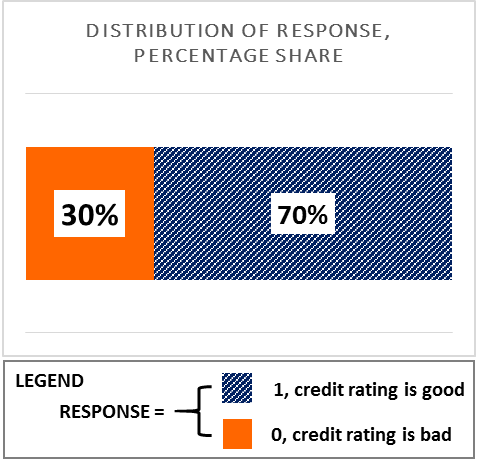
\includegraphics[width=0.4\textwidth]{response.png}
	\caption{Distribution of $RESPONSE$, percentage share, n=1.000 observations}
	\label{response}
\end{figure}\\
In figure \ref{categoricals} we can see the distribution of $RESPONSE$ by all other categorical variables $CHECK\_ACC$, $HISTORY$, $SAV\_ACCT$, $PRESENT\_RESIDENT$, $EMPLOYMENT$, and $JOB$. According to \cite[pp.76-77]{shmueli} categorical variables can inflate the dimension of the dataset which we can see by comparing the original dataset which had 20 variables in total and the preprocessed data set which has 32 variables (due to categorical and binary variables). The preprocessing however is necessary in order to be able to conduct data mining methods on the data set. \cite[pp.76-77]{shmueli} suggest to reduce the number of sub-categories through combination of similar sub-categories. 

Regarding the distribution of $RESPONSE$ by $CHECK\_ACC$ there are four sub-categories with each having different distributions so that combining categories would not be a good choice. Sub-category \textit{0:< 0 DM} is the worst and sub-category \textit{3:no checking account} is the best according to the given data set. Putting the attribute \textit{3:no checking account} as best outcome is strange because if there is no checking account then for instance a bank does not have any business and therefore it is actually a rather bad attribute. Since we do not have domain knowledge the order of $CHECK\_ACC$ will be kept as it is.

Looking at the distribution of $RESPONSE$ by $HISTORY$ there are five sub-categories with categories \textit{0:no credits taken} and \textit{1:all credits at this bank paid back} as well as \textit{2:existing credits paid back duly} and \textit{3:delay in paying off in the past} having similar distributions. With respect to their similarities in distribution these two pairs of categories could be combined, however with regard to the rather different attributional message of these variables as well as the missing domain knowledge, these variables are not combined. Regardless of this the order has to be reversed to stay constistent with $CHECK\_ACC$ (and for the interpretation) because the worst attribute is assigned the best category at the moment. With regard to $SAV\_ACCT$ there is the same issue as with $HISTORY$. Here two categories \textit{0:< 100 DM} and \textit{1:100$\leq$..<500 DM} can be combined as well as the three other categories. However since each sub-category describes different attributions and due to missing domain knowledge the order will be kept as it is. 

Regarding $PRESENT\_RESIDENT$ all four sub-categories have a similar distribution which leads to the assumption that they could be combined. However combining these categories would create a non-sense category. Furthermore there is an error in the data set regarding this variable with respect to the inconsistency of the coding which starts at 0 and ends with 3. The raw data set however starts with the value 1 and ends with the value 4. We could assume that during the transformation process the values were shiftet by 1 unit. Since it is not retraceable how the error occured we decide to omitt this variable for the later analysis.

The variable $EMPLOYMENT$ is sub-divided into five sub-categories with each having a slightly different distribution. We decide not to combine categories in this category because a long employment status implies higher income security and thus it makes sense to leave the categories as they are.
\begin{figure}[htbp]
	\centering
	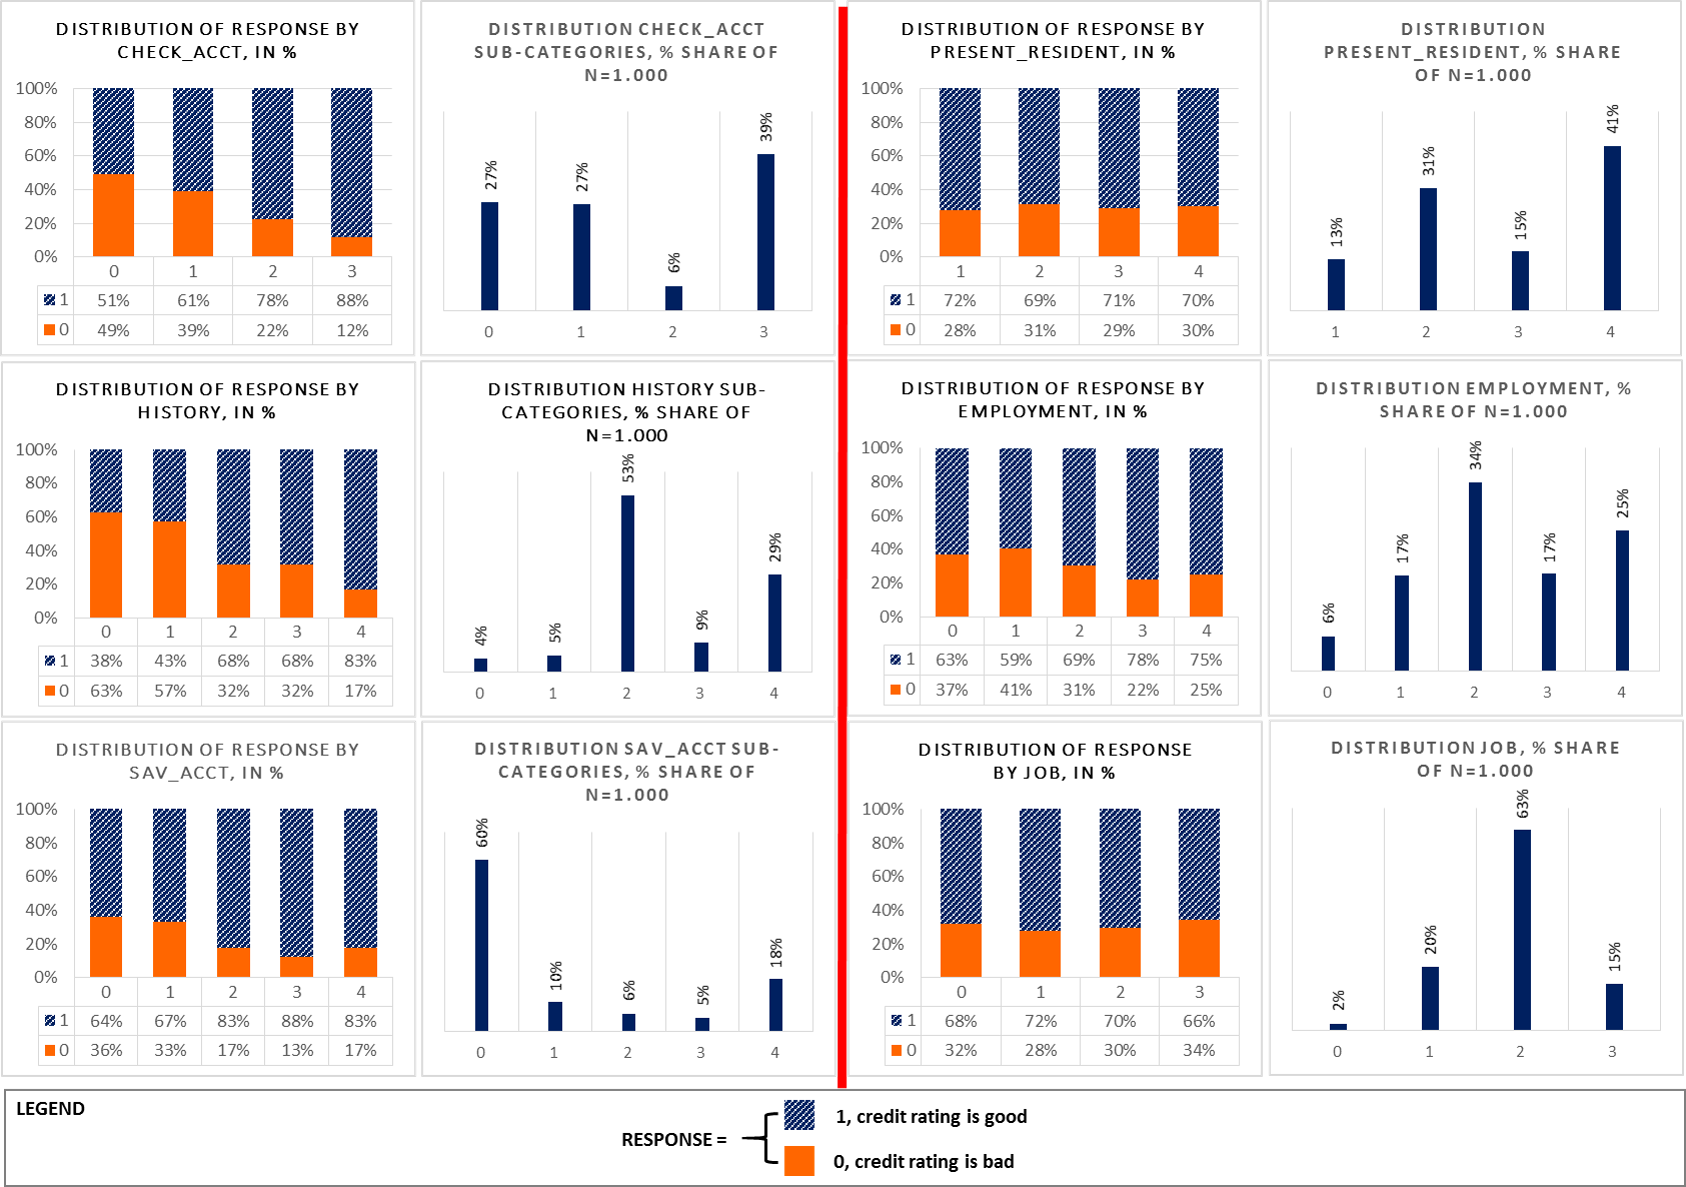
\includegraphics[width=0.7\textwidth]{categoricals.png}
	\caption{Distribution of $RESPONSE$ with other Categorical variables, percentage share of sub-categories of each category, n=1.000}
	\label{categoricals}
\end{figure}
\begin{figure}[!]
	\centering
	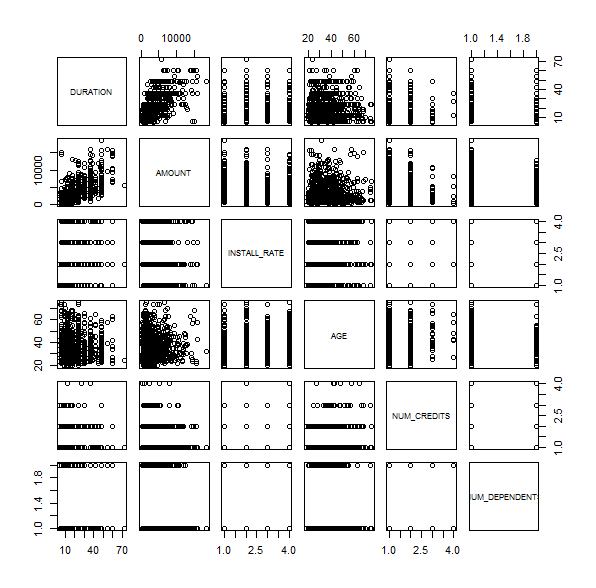
\includegraphics[width=\textwidth]{scatterplot.png}
	\caption{Title}
	\label{scatterplot}
\end{figure}
\newpage
In figure \ref{corrMatrix} the correlation matrix of the German Credit data set is displayed in percentage.
\begin{figure}[!]
	\centering
	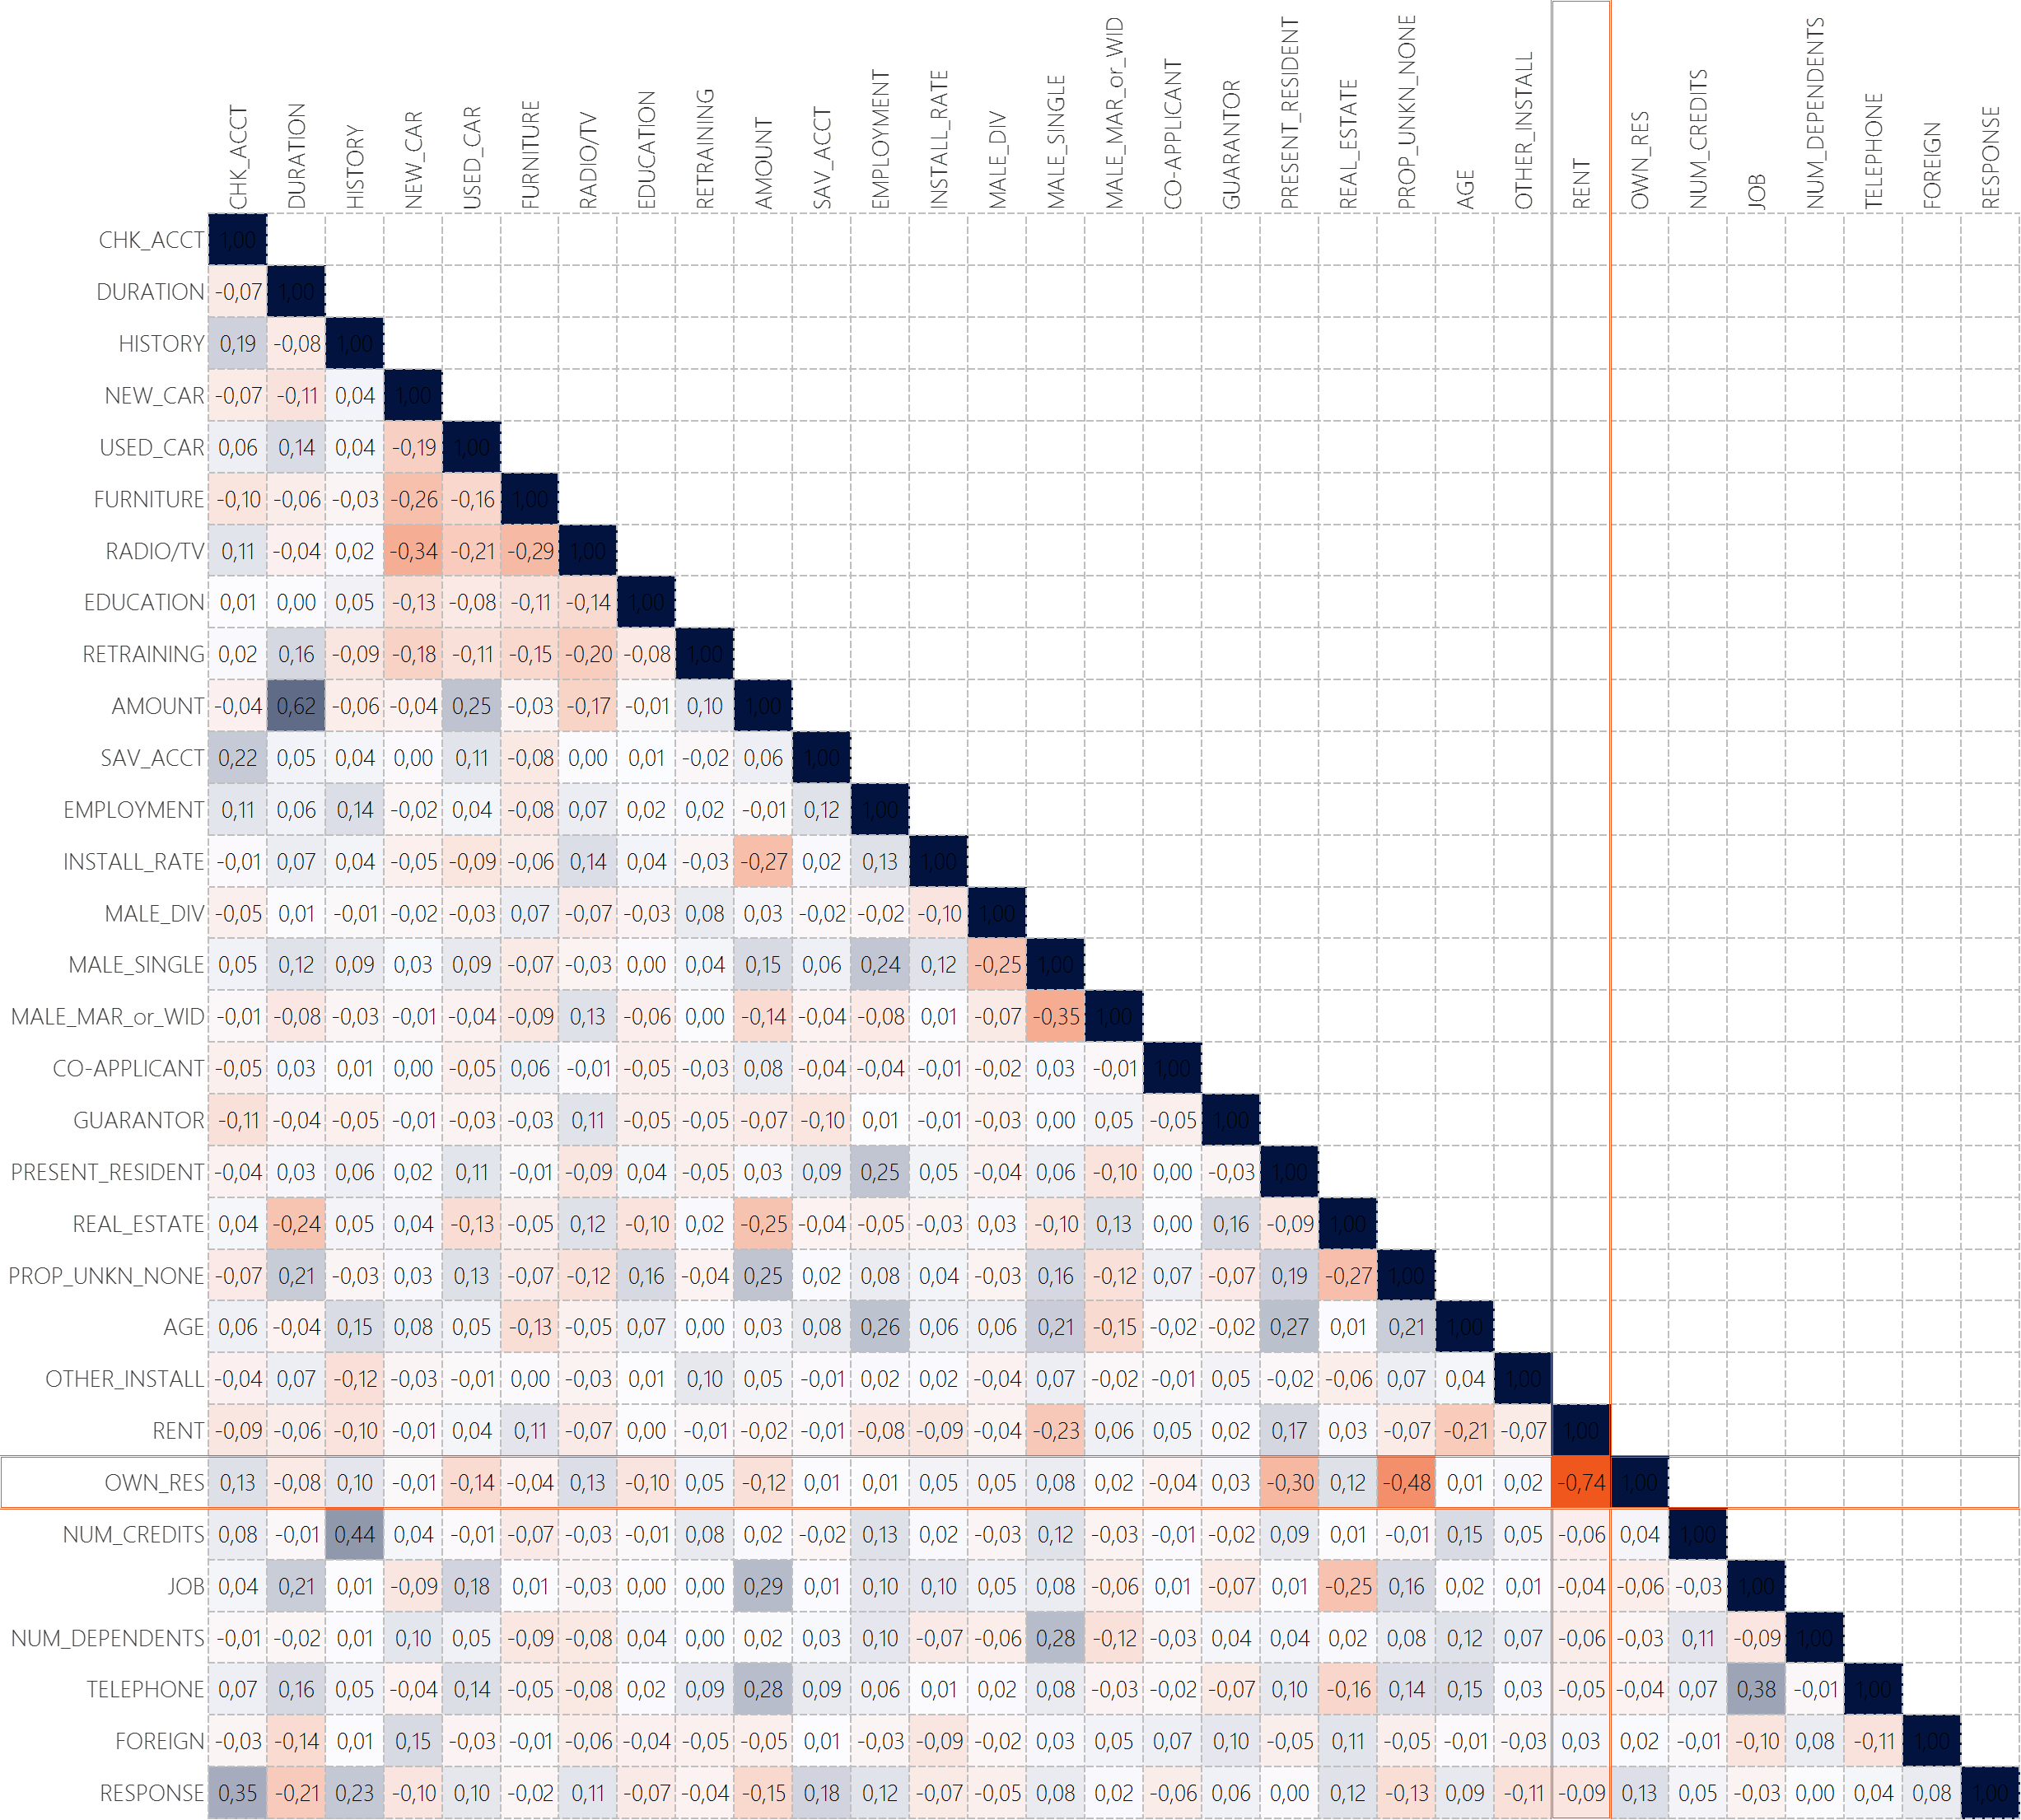
\includegraphics[width=\textwidth]{CorrPlot.png}
	\caption{Correlation Matrix of German Credit Data Set, in \%}
	\label{corrMatrix}
\end{figure}
\begin{table}[]
	\centering
	\caption{Statistical Overview of German Credit Data Set, n=1.000}
	\label{overview}
	\begin{tabular}{|l|l|l|l|l|l|l|l|l|l|l|l|l|l|l|}\hline
		{\tiny \textbf{Variable}} & {\tiny \textbf{Av. Value}} & {\tiny \textbf{Standard Error}} & {\tiny \textbf{Median}}   & {\tiny \textbf{Modus}}& \begin{tabular}[c]{@{}l@{}}{\tiny \textbf{Standard}}\\{\tiny \textbf{Deviation}}\end{tabular} & \textbf{{\tiny Sample Variance}} & {\tiny \textbf{Curtosis}} & \textbf{\textbf{Skewness}} & {\tiny \textbf{Value Range}} & {\tiny \textbf{Minimum}} & {\tiny \textbf{Maximum}}   & {\tiny \textbf{Sum }}         & \textbf{{\tiny Count}}    & \textbf{{\tiny Confidence Level}} \\\hline
		{\tiny OBS\#}&{\tiny 500,50 }&{\tiny 9,13}&{\tiny 500,50}&{\tiny \#N/A }&{\tiny 288,82}&{\tiny 83.416,67}&{\tiny (1,20)}&{\tiny (0,00)}&{\tiny 999,00}&{\tiny 1,00}&{\tiny 1.000,00}&{\tiny 500.500,00}&{\tiny 1.000,00}&{\tiny 17,92}\\ \hline
		{\tiny CHK\_ACCT}& 1,58      & 0,04           & 1,00     & 3,00     & 1,26                                                           & 1,58               & (1,66)   & 0,01     & 3,00        & -       & 3,00      & 1.577,00     & 1.000,00 & 0,08             \\
		{\tiny DURATION}& 20,90     & 0,38           & 18,00    & 24,00    & 12,06                                                          & 145,42             & 0,92     & 1,09     & 68,00       & 4,00    & 72,00     & 20.903,00    & 1.000,00 & 0,75             \\
		{\tiny HISTORY}& 2,55      & 0,03           & 2,00     & 2,00     & 1,08                                                           & 1,17               & (0,58)   & (0,01)   & 4,00        & -       & 4,00      & 2.545,00     & 1.000,00 & 0,07             \\
		{\tiny NEW\_CAR}& 0,23      & 0,01           & -        & -        & 0,42                                                           & 0,18               & (0,42)   & 1,26     & 1,00        & -       & 1,00      & 234,00       & 1.000,00 & 0,03             \\
		{\tiny USED\_CAR}& 0,10      & 0,01           & -        & -        & 0,30                                                           & 0,09               & 4,85     & 2,62     & 1,00        & -       & 1,00      & 103,00       & 1.000,00 & 0,02             \\
		{\tiny FURNITURE}& 0,18      & 0,01           & -        & -        & 0,39                                                           & 0,15               & 0,76     & 1,66     & 1,00        & -       & 1,00      & 181,00       & 1.000,00 & 0,02             \\
		{\tiny RADIO/TV}& 0,28      & 0,01           & -        & -        & 0,45                                                           & 0,20               & (1,04)   & 0,98     & 1,00        & -       & 1,00      & 280,00       & 1.000,00 & 0,03             \\
		{\tiny EDUCATION}& 0,05      & 0,01           & -        & -        & 0,22                                                           & 0,05               & 15,13    & 4,14     & 1,00        & -       & 1,00      & 50,00        & 1.000,00 & 0,01             \\
		{\tiny RETRAINING}& 0,10      & 0,01           & -        & -        & 0,30                                                           & 0,09               & 5,45     & 2,73     & 1,00        & -       & 1,00      & 97,00        & 1.000,00 & 0,02             \\
		{\tiny AMOUNT}& 3.271,26  & 89,26          & 2.319,50 & 1.393,00 & 2.822,74                                                       & 7.967.843,47       & 4,29     & 1,95     & 18.174,00   & 250,00  & 18.424,00 & 3.271.258,00 & 1.000,00 & 175,16           \\
		{\tiny SAV\_ACCT}& 1,11      & 0,05           & -        & -        & 1,58                                                           & 2,50               & (0,68)   & 1,02     & 4,00        & -       & 4,00      & 1.105,00     & 1.000,00 & 0,10             \\
		{\tiny EMPLOYMENT}& 2,38      & 0,04           & 2,00     & 2,00     & 1,21                                                           & 1,46               & (0,93)   & (0,12)   & 4,00        & -       & 4,00      & 2.384,00     & 1.000,00 & 0,07             \\
		{\tiny INSTALL\_RATE}& 2,97      & 0,04           & 3,00     & 4,00     & 1,12                                                           & 1,25               & (1,21)   & (0,53)   & 3,00        & 1,00    & 4,00      & 2.973,00     & 1.000,00 & 0,07             \\
		{\tiny MALE\_DIV}& 0,05      & 0,01           & -        & -        & 0,22                                                           & 0,05               & 15,13    & 4,14     & 1,00        & -       & 1,00      & 50,00        & 1.000,00 & 0,01             \\
		{\tiny MALE\_SINGLE}& 0,55      & 0,02           & 1,00     & 1,00     & 0,50                                                           & 0,25               & (1,97)   & (0,19)   & 1,00        & -       & 1,00      & 548,00       & 1.000,00 & 0,03             \\
	{\tiny 	MALE\_MAR\_or\_WID}& 0,09      & 0,01           & -        & -        & 0,29                                                           & 0,08               & 6,01     & 2,83     & 1,00        & -       & 1,00      & 92,00        & 1.000,00 & 0,02             \\
		{\tiny CO-APPLICANT}& 0,04      & 0,01           & -        & -        & 0,20                                                           & 0,04               & 19,54    & 4,64     & 1,00        & -       & 1,00      & 41,00        & 1.000,00 & 0,01             \\
		{\tiny GUARANTOR}& 0,05      & 0,01           & -        & -        & 0,22                                                           & 0,05               & 14,36    & 4,04     & 1,00        & -       & 1,00      & 52,00        & 1.000,00 & 0,01             \\
		{\tiny PRESENT\_RESIDENT}& 2,85      & 0,03           & 3,00     & 4,00     & 1,10                                                           & 1,22               & (1,38)   & (0,27)   & 3,00        & 1,00    & 4,00      & 2.845,00     & 1.000,00 & 0,07             \\
		{\tiny REAL\_ESTATE}& 0,28      & 0,01           & -        & -        & 0,45                                                           & 0,20               & (1,06)   & 0,97     & 1,00        & -       & 1,00      & 282,00       & 1.000,00 & 0,03             \\
		{\tiny PROP\_UNKN\_NONE}& 0,15      & 0,01           & -        & -        & 0,36                                                           & 0,13               & 1,69     & 1,92     & 1,00        & -       & 1,00      & 154,00       & 1.000,00 & 0,02             \\
		{\tiny AGE}& 35,55     & 0,36           & 33,00    & 27,00    & 11,38                                                          & 129,40             & 0,60     & 1,02     & 56,00       & 19,00   & 75,00     & 35.546,00    & 1.000,00 & 0,71             \\
		{\tiny OTHER\_INSTALL}& 0,19      & 0,01           & -        & -        & 0,39                                                           & 0,15               & 0,61     & 1,62     & 1,00        & -       & 1,00      & 186,00       & 1.000,00 & 0,02             \\
		{\tiny RENT}& 0,18      & 0,01           & -        & -        & 0,38                                                           & 0,15               & 0,81     & 1,68     & 1,00        & -       & 1,00      & 179,00       & 1.000,00 & 0,02             \\
		{\tiny OWN\_RES}& 0,71      & 0,01           & 1,00     & 1,00     & 0,45                                                           & 0,20               & (1,11)   & (0,94)   & 1,00        & -       & 1,00      & 713,00       & 1.000,00 & 0,03             \\
		{\tiny NUM\_CREDITS}& 1,41      & 0,02           & 1,00     & 1,00     & 0,58                                                           & 0,33               & 1,60     & 1,27     & 3,00        & 1,00    & 4,00      & 1.407,00     & 1.000,00 & 0,04             \\
		{\tiny JOB}& 1,90      & 0,02           & 2,00     & 2,00     & 0,65                                                           & 0,43               & 0,50     & (0,37)   & 3,00        & -       & 3,00      & 1.904,00     & 1.000,00 & 0,04             \\
		{\tiny NUM\_DEPENDENTS}& 1,16      & 0,01           & 1,00     & 1,00     & 0,36                                                           & 0,13               & 1,65     & 1,91     & 1,00        & 1,00    & 2,00      & 1.155,00     & 1.000,00 & 0,02             \\
		{\tiny TELEPHONE}& 0,40      & 0,02           & -        & -        & 0,49                                                           & 0,24               & (1,85)   & 0,39     & 1,00        & -       & 1,00      & 404,00       & 1.000,00 & 0,03             \\
		{\tiny FOREIGN }& 0,04      & 0,01           & -        & -        & 0,19                                                           & 0,04               & 22,18    & 4,91     & 1,00        & -       & 1,00      & 37,00        & 1.000,00 & 0,01             \\
		{\tiny RESPONSE}& 0,70      & 0,01           & 1,00     & 1,00     & 0,46                                                           & 0,21               & (1,24)   & (0,87)   & 1,00        & -       & 1,00      & 700,00       & 1.000,00 & 0,03\\ \hline            
	\end{tabular}
\end{table}
